\documentclass{article}

\title{Lab-3}
\author{2347139}
\date{\today}


\usepackage{listings}
\usepackage{color}
\usepackage{graphicx}

\definecolor{dkgreen}{rgb}{0,0.6,0}
\definecolor{gray}{rgb}{0.5,0.5,0.5}
\definecolor{mauve}{rgb}{0.58,0,0.82}

\lstset{frame=tb,
  language=Java,
  aboveskip=3mm,
  belowskip=3mm,
  showstringspaces=false,
  columns=flexible,
  basicstyle={\small\ttfamily},
  numbers=left,
  numberstyle=\tiny\color{gray},
  keywordstyle=\color{blue},
  commentstyle=\color{dkgreen},
  stringstyle=\color{mauve},
  breaklines=true,
  breakatwhitespace=true,
  tabsize=3
}
\begin{document}
\maketitle
\begin{lstlisting}
    // Implement the concept of Nested class, Inner Class, String class & String
    // Buffer Class in a single program based on your domain.
    
    // 1.Since String is immutable in Java, whenever we do String manipulation like concatenation, substring, etc. it generates a new String and discards the older String for garbage collection.
    
    class Guild {
        public String botName;
        protected String discordToken;
    
        Guild(String botName, String discordToken) {
            if (discordToken.isEmpty()) {
                System.out.println("Token not found");
            }
            this.botName = botName;
            this.discordToken = discordToken;
        }
    
        public void showBotDetails() {
            System.out.println("Discord Bot with " + botName + " created in your account");
    
        }
    
        public void createGuild(String guildName) {
            System.out.println("Created a guild " + guildName + " associated to the bot");
        }
    
        public void getBotPermission(int permission) {
            boolean isAdmin = true;
            boolean isMod = true;
            boolean BAN_MEMBERS = true;
            boolean KICK_MEMBERS = true;
            if (permission == 0) {
                System.out.println("The Bot created has 0 permission");
            }
            if (isAdmin && isMod && BAN_MEMBERS && KICK_MEMBERS) {
                System.out.println("The Bot is set full permission");
            }
    
        }
    
        public void showBotDetails(String clientName) {
            System.out.println("Discord Bot with " + botName + " created for client" + clientName);
        }
    
        class SlashCommands { // inner class
            public void getMembers() {
                System.out.println("Getting members of the text channel");
                System.out.println("Channel members are : Elumeveguy\n" + //
                        "Emojorekes\n" + //
                        "Eroxihisom\n" + //
                        "Ulelabutuk\n" + //
                        "Ayibiciqeb\n" + //
                        "Oguyocuxas\n" + //
                        "Uxibabujen\n" + //
                        "Epiwimaguk\n" + //
                        "Idenefibiy\n" + //
                        "Amarebamat");
    
            }
    
            public void slashCommand(StringBuffer user) {
                // String command='ban';
                System.out.println("Ban User ");
                System.out.println("user " + user + " is banned");
    
            }
        }
    
        static class Client { // nested class
            public String name;
            public String discordServer;
    
            public void getClient(String name, String discordServer) {
                this.name = name;
                this.discordServer = discordServer;
            }
    
            public void getBotDetails() {
                System.out.println("your account name is " + name);
                System.out.println("your Discord server name is " + discordServer);
    
            }
        }
    
    }
    
    class Main {
        public static void main(String args[]) {
            StringBuffer bf = new StringBuffer("bob");
            Guild build = new Guild("bot- Mointer", "3836958915");
            build.showBotDetails();
            build.createGuild("Mointer");
            build.getBotPermission(0);
    
            Guild.SlashCommands sl = build.new SlashCommands();
            sl.getMembers();
            sl.slashCommand(bf);
    
            Guild.Client client;
            client = new Guild.Client();
            client.getClient("john", "john's server");
            client.getBotDetails();
    
        }
    }
\end{lstlisting}

\section*{Output}
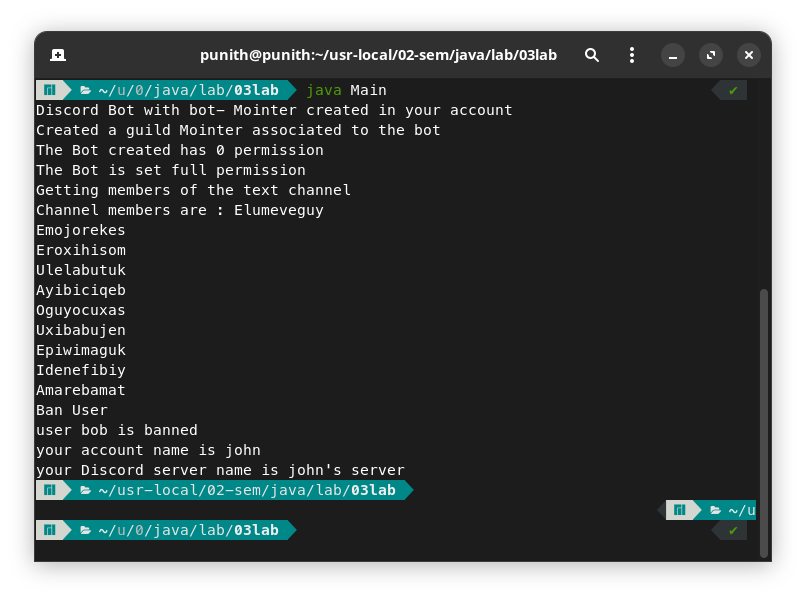
\includegraphics[width=11cm, height=9cm]{./images/01.png}

\end{document}
